Pour les formules mathématiques de réfractions nous avons utiliser celle sur le site \href{https://www.scratchapixel.com/lessons/3d-basic-rendering/introduction-to-shading/reflection-refraction-fresnel}{scratchapixel}.
Les materiaux utilisant de la transparance ont un paramètres supplémentaire : l'indice de réfraction. Pour nos tests nous avons pris celui donnée par wikipedia pour le pyrex(1,474). Nous avions au départ mis un parametre pour savoir à quel point le materiaux était refractif ou non, mais nous l'avons remplacé par l'equation de fresnel qui calcul la proportion de lumière qui est réfléchie / réfractée. Cette proportion change en fonction de l'angle de pénétration de l'objet, d'où la nécéssité de l'emploi de la formule.

\begin{figure}[h]
   \begin{center}
       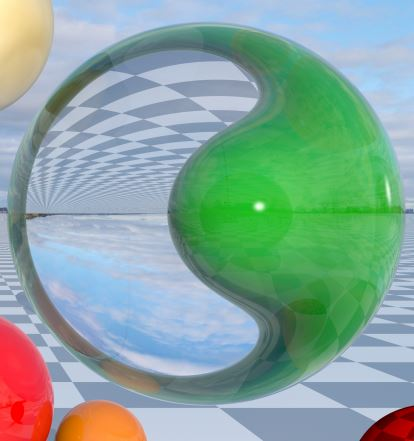
\includegraphics[scale=0.8]{img/rt/refractions.jpg}
   \end{center}
   \caption{Nous pouvons observer une boule verte à travers la boule transparente ainsi que le paysage qui est inversé à cause de la refraction}
\end{figure}
